\section{LoRa}

Before analysing IoT systems more generally, I will explain the most critical
hardware enabling technology for this project which is the radio communication
technique known as LoRa.

\subsection{What is LoRa?}

LoRa stands for \textbf{Lo}ng \textbf{Ra}nge and it is a radio modulation
technique invented in 2014 that allows for the transmission of data over very
long distances. It is one of several competing low power wide area networks
(LPWAN) but the hardware to use it is much more widespread than these other
networks. Compared to WiFi, LoRa has a range over 4000 times greater
\cite{spiess2019}. The world record distance for a LoRa signal is 1336km
\cite{ttn2023}. This was achieved under abnormal conditions: a fishing boat near
Portugal with a LoRa transmitter had one of its packets received on the high
altitude Canary islands. This exceptional range is also achieved with remarkably
little power.

\subsection{How LoRa works}

As this paper is not a technical study of radio communication I will opt for a
brief summary of the principles behind LoRa. With this in mind I have based much
of the information from the excellent video lecture in \cite{visualelectric2021}
that itself draws upon the paper in \cite{vangelista2017}.

The reason LoRa modulation is different to traditional modulation techniques is
the use of a "chirp" as the key to transmitting packets. A more traditional
technique might involve a frequency shift key; that is a single frequency
represents several bits. These unique frequencies are called symbols as they
represent data, like letters in the alphabet. In the below graph we see three
simplified symbols that represent binary values, the combination of these
symbols makes a packet:

\begin{figure}[H]
  \centering
  % left image
  \begin{minipage}{0.48\textwidth}
    \centering
    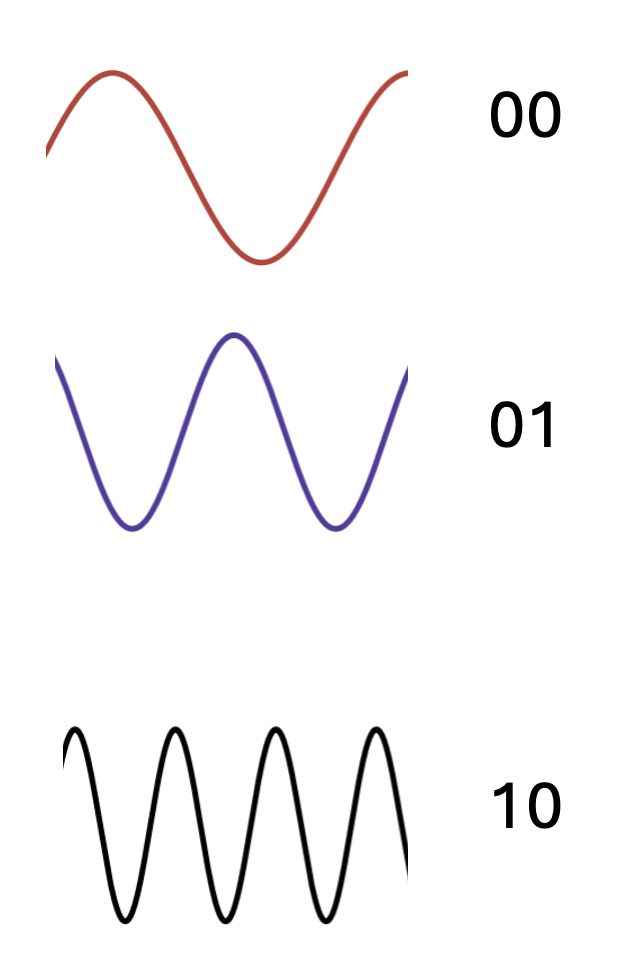
\includegraphics[width=0.4\linewidth]{contents/part-1/fig1/frequencysymbols.png}
    \\[4pt]
    {\small (a) Frequency shift symbols} \end{minipage}\hfill
  % right image
  \begin{minipage}{0.48\textwidth}
    \centering
    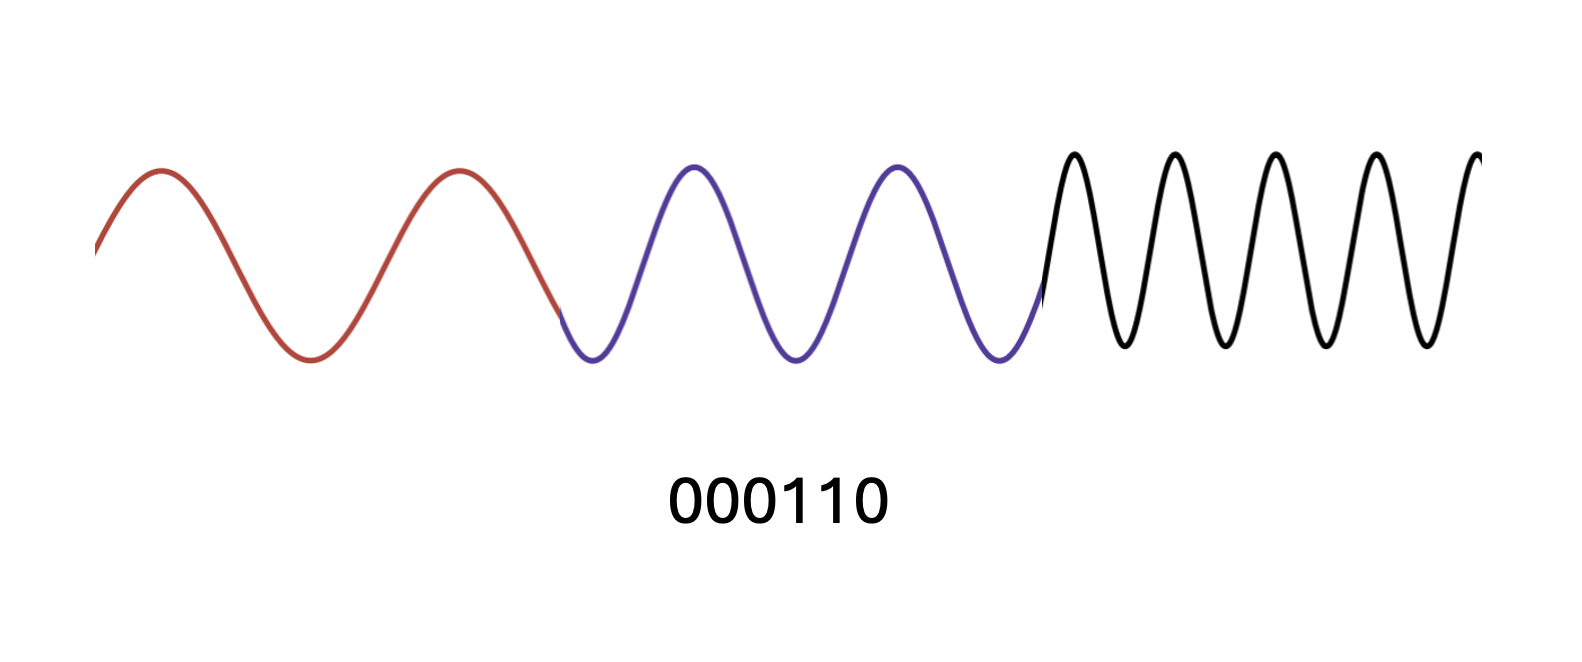
\includegraphics[width=1\linewidth]{contents/part-1/fig1/packet.png}
    \\[4pt]
    {\small (b) Packet}
  \end{minipage}
  \caption{ Traditional radio modulation with frequency symbols}
  \label{fig:freq-and-packet}
\end{figure}

In traditional modulation, symbols always have flat unchanging frequency (as can
be seen from the fact the wave separation never changes). LoRa symbols instead
have changing frequencies that have a waveform like the below.

\begin{figure}[H]
    \centering
    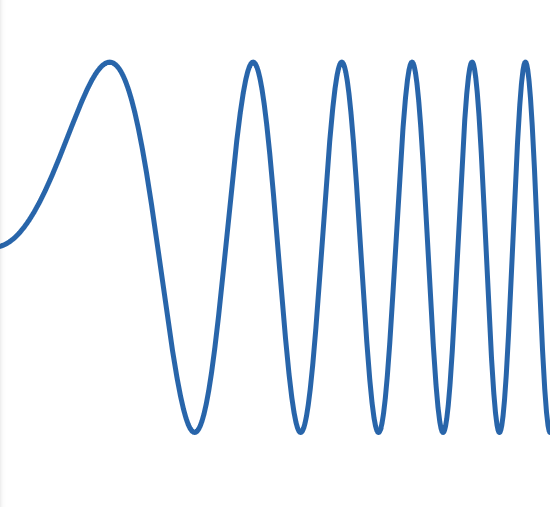
\includegraphics[width=0.15\textwidth]{contents/part-1/fig1/lorawavelength.png}
    \caption{LoRa symbol showing changing frequency ("Up-chirp")}
    \label{fig:lora-wave}
\end{figure}

This change in frequency is what gives the wave form the name "chirp". If
traditional frequency symbols were thought of a sound they would be similar to
morse code beeps while LoRa would be more similar to siren or \textit{chirp}ing
bird. LoRa has both rising and falling chirps (up-chirps and down-chirps).

Different LoRa symbols are then distinguished by the point in time of a
discontinuity. LoRa symbols are always delivered over a known length of time, so
different symbols include a reset back to the starting frequency at a different
point in time.

A way to graphically show this discontinuity in LoRa and compare it to frequency
shift modulation is by using instantaneous frequency graphs:

\begin{figure}[H]
  \centering
  % left image
  \begin{minipage}{0.48\textwidth}
    \centering
    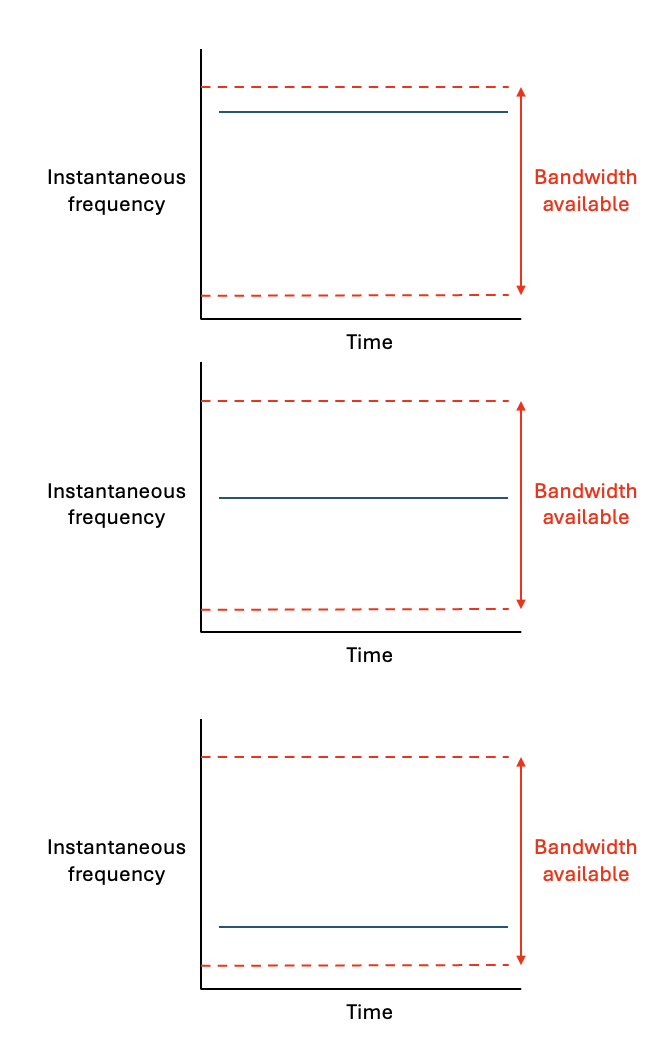
\includegraphics[width=0.9\linewidth]{contents/part-1/fig1/traditional-wavechart.png}
    \\[4pt]
    {\small (a) Frequency shift symbols} \end{minipage}\hfill
  % right image
  \begin{minipage}{0.48\textwidth}
    \centering
    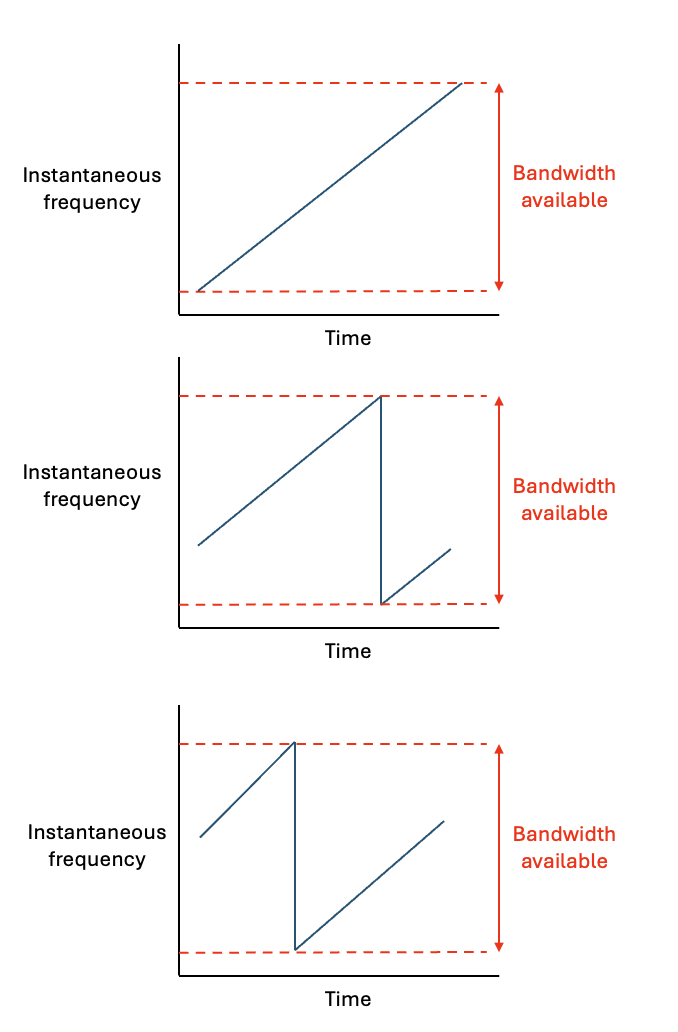
\includegraphics[width=0.9\linewidth]{contents/part-1/fig1/lora-wavechart.png}
    \\[4pt]
    {\small (b) LoRa symbols, note shifting discontinuity}
  \end{minipage}
  \caption{ Comparison of frequency shift and LoRa modulation }
  \label{fig:freq-vs-lora}
\end{figure}

Once these symbols hit the receiver, the receiver must work out which symbol it
was. In frequency shift modulation this is achieved by performing a correlation
test against every symbol received. However this is computationally difficult
and requires a low signal-to-noise ratio to work effectively. The benefit of
chirps is that due to a mathematical transformation that will not be further
discussed (Fast Fourier transform), the correlation can be computed much more
easily and with less powerful hardware.

\subsection{Benefits and limitations}\label{sec:lora-benefits}

The benefits from the ability of the LoRa receiver to demodulate signals more
efficiently is two-fold. First it reduces the power needs on transmitter and
receiver: the transmitter sends less powerful signals because the receiver can
more easily distinguish signals; in turn the receiver can also demodulate with a
lower power budget because of the easier correlation process with LoRa chirps.

The second related benefit is the ability for the receiver to demodulate signals
which are below the noise floor (the sum of all interfering signals).
Essentially, even when background noise is 'louder' than the LoRa signal, the
receiver is still able to distinguish and process the data in the signal. This
helps LoRa transmitters to broadcast signals with a far greater effective range
despite it's low power. 

\begin{table}[ht]
  \centering
  \begin{tabular}{|l|l|p{4.5cm}|r|}
    \hline
\textbf{Technology} & \textbf{Wireless Communication} & \textbf{Range} &
\textbf{Tx Power} \\
    \hline
    Bluetooth & Short range & 10 m & 2.5 mW \\
    \hline
    WiFi & Short range & 50 m & 80 mW \\
    \hline
    3G/4G & Mobile network & 5,000m & 5000 mW \\
    \hline
    LoRa & LPWAN & \parbox[t]{4.5cm}{2,000--15,000m} & 20 mW \\
    \hline
  \end{tabular}
    \caption{Comparison of wireless technologies (Source:
  \cite{lie_lora_readthedocs})}
\end{table}
